\subsection{Naive Bayes SVM}

In order to find effective text classification methods, we explored the Naive Bayes-Support Vector Machine (NB-SVM) model, inspired by the insights from the paper ``Baselines and Bigrams: Simple, Good Sentiment and Topic Classification.'' This hybrid model combines the probabilistic foundations of Naive Bayes with the robustness of Support Vector Machines, making it particularly suitable for complex text classification tasks like toxic comment classification.


\subsubsection{Model Description}
In our implementation, we opted for Logistic Regression as a proxy for SVM, owing to its effectiveness in similar contexts. This combination aims to leverage the feature selection capabilities of Naive Bayes and the optimization strengths of SVM.

\subsubsection{Implementation Steps}
Our implementation of NB-SVM involved the following key steps:

\begin{enumerate}
  \item \textbf{TF-IDF Vectorization}: We transformed the text data into TF-IDF vectors with an ngram range of 1 to 2. This allowed us to capture both the significance of individual words (unigrams) and their contextual relationships (bigrams).
  
  \item \textbf{Naive Bayes Probability Computation}: \\
  For each label, we computed the log ratio of probabilities, $R = \log\left(\frac{P_{NB}(y = 1)}{P_{NB}(y = 0)}\right)$, where $P_{NB}$ denotes the Naive Bayes probability. This ratio reflects the relative importance of each feature for the respective label.
  
  \item \textbf{Recomputing TF-IDF Values with Naive Bayes}: The TF-IDF values were multiplied by the computed $R$ values, effectively reweighting them in accordance with their importance in class differentiation. We trained a Logistic Regression model for each label using the recomputed TF-IDF.

  \item \textbf{Tuning Regularization $C$}: We fine tuned the regularization parameter $C$, to identify which value would provide us with the best performing model. We finally chose the value: 0.5. Refer graph \ref{fig:enter-label} for improvement of the model for each label for various values of $C$.
\end{enumerate}

\begin{figure}
    \centering
    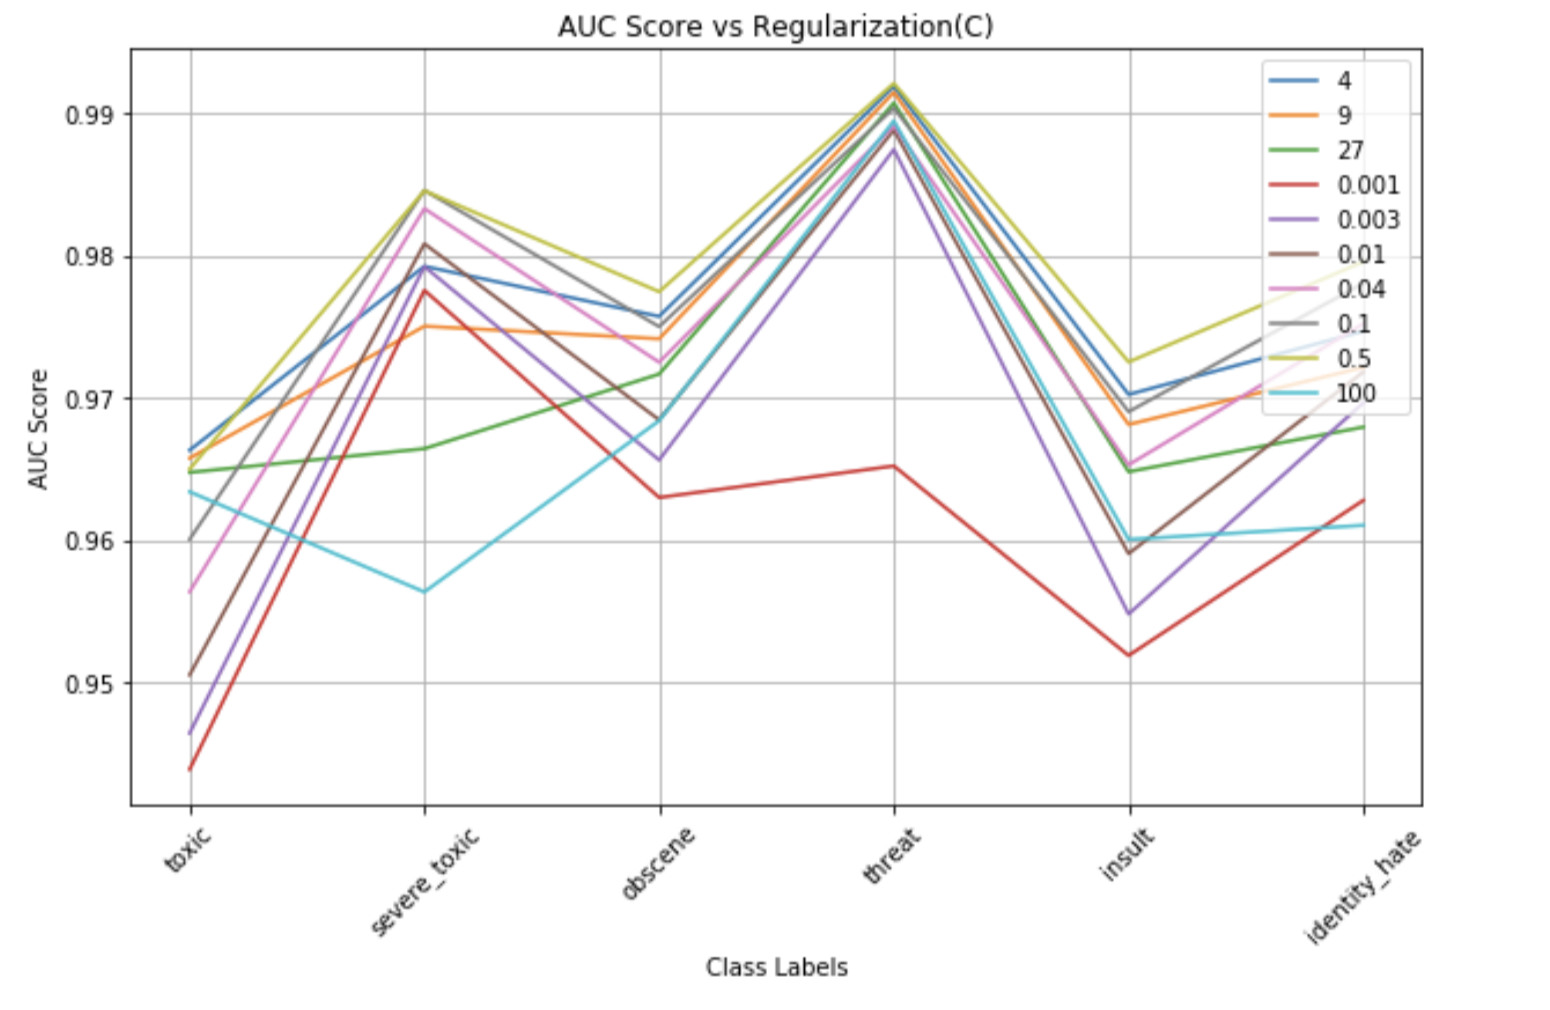
\includegraphics[scale=0.5]{images/graphs/Reg_AUC.png}
    \caption{Tuning Regularization ($C$) over label vs AUC score}
    \label{fig:enter-label}
\end{figure}


\subsubsection{Results and Evaluation}
The performance of the NB-SVM model was assessed using a suite of metrics, including precision, recall, F1 score, accuracy, and ROC-AUC. These metrics collectively provided a comprehensive view of the model's efficacy across various aspects of classification.  Table \ref{tab:model_metrics_nbsvm} shows the test accuracy, AUC Score, F1 Score, Precision and Recall per label and also the weighted average.

\begin{table}[h]
\centering
\begin{tabular}{|c|c|c|c|c|c|}
\hline
 & Test Accuracy (\%) & AUC Score (\%) & F1 Score (\%) & Precision (\%) & Recall (\%) \\
\hline
toxic & 93.35 & 96.63 & 69.00 & 94.21 & 93.35 \\
severe\_toxic & 99.27 & 97.92 & 35.26 & 99.26 & 99.27 \\
obscene & 96.65 & 97.57 & 69.93 & 96.55 & 96.65 \\
threat & 99.72 & 99.19 & 44.85 & 99.66 & 99.72 \\
insult & 96.56 & 97.02 & 62.67 & 96.22 & 96.56 \\
identity\_hate & 99.09 & 97.47 & 43.05 & 98.91 & 99.09 \\
\hline
\textbf{Weighted Avg.} & \textbf{95.47} & \textbf{97.07} & \textbf{65.26} & \textbf{95.72} & \textbf{95.47} \\
\hline
\end{tabular}
\caption{Model Evaluation Metrics for NBSVM}
\label{tab:model_metrics_nbsvm}
\end{table}


\subsubsection{Conclusion}
The NBSVM model showcases an effective way to combine the strengths of Naive Bayes and SVM in text classification. Our implementation for the toxic comment classification task underscores its potential in dealing with nuanced data. Future endeavors may include further model parameter tuning, exploring alternative feature extraction techniques, or integrating NBSVM with advanced models like neural networks for enhanced performance.







